\hypertarget{chap:method}{\chapter{Method}}\label{method}
In this section, we introduce our methods for improving the accuracy of sentiment classification task on \hyperref[sec:sst]{Stanford Sentiment Treebank dataset with binary setting}.
In search of new improvements, we have tried three different approaches:
\begin{description}
\item[\deschyperlink{sec:VTtree}{Utilizing local syntactic information at each node of Recursive Neural Networks}] The first approach is mainly based on the success of Tag Embeddings Recursive Neural Networks~\cite{tag-embedding-rnn}.
In this paper, the authors parameterized the composition functions at each parse tree's node with respect to the grammar rule expanding that node. 
By doing so, the authors was able to not only efficiently improve the performance of RNTN (Socher, 2013)~\cite{socher2013recursive} (from \(85.4\%\) to \(87.7\%\) accuracy) but also their models used much smaller number of parameters \((54K)\) compared to that of RNTN \((108K)\)~\cite{tag-embedding-rnn}.
Given the success of \hyperref[sec:treelstm]{Tree-LSTM models}, we hypothesized that by parameterized the composition functions of a Tree-LSTMs unit at a node with respect to the grammar rule expanding that node, we can improve the performance of Tree-LSTMs (in the same way how this method improving RNTN).

\textbf{This approach was later proven to be unsuccessful}, so we tried two more different approaches.

\item[\deschyperlink{sec:Glove-Amazon}{Transfer Learning by retraining Glove on Amazon Reviews dataset}] \label{movie-hypothesis} There are many words (e.g. "B-rated", "Batman", "Nolan", "cartoonlike") which rarely appears in regular documents but more often in movie reviews.
We hypothesized that by training word embeddings of review documents, especially movie or book reviews, we can capture more rare words and also the different way people use words (or different word relationships) to express their opinions on movies or books.
For archiving these purposes, we retrained Glove vectors~\cite{glove} on part of  \hyperref[sec:amazon]{Amazon Reviews dataset}.
This new Glove vectors was named Glove Amazon.
For evaluating Glove Amazon, we replaced the Glove Common Crawl\footnote{Common Crawl (840B tokens, 2.2M vocab, cased, 300d vectors, 2.03 GB download) publicly available at \url{https://nlp.stanford.edu/projects/glove/}} with Glove Amazon for initializing Tree-LSTMs' word embedding layer.

\textbf{In spite of being a simple method, it dramatically improves Tree-LSTMs performance.}
This is our first successful method for transfer learning from document-level (Amazon Reviews) to sentence-level labeled dataset (Stanford Sentiment Treebank).
Inspired by this method, we cooperated it into the development of our next approach.

\item[\deschyperlink{sec:CNNtree}{Combining Recusive Neural Networks with Convolution Neural Networks}] \label{conv-tree-benefits} Based on our discussion on tree-structured versus sequential network architects (Sec.\ref{sec:tree-discuss}) and the benefits of using convolution layer (Sec.\ref{kim-cnn}), we combined Convolution Neural Networks with Tree-LSTM and \hyperref[sec:lstm]{sequential LSTM}.
We hypothesized that the convolution layer will help Tree-LSTMs to mitigate the problem of lacking local context and weak feature capturing at leaf nodes (Sec.\ref{sec:tree-discuss}).
Additionally, using Tree-LSTM to combine the feature maps produced by convolution layer is better than max-over-time pooling layer (Sec.\ref{kim-drawback}).
The increased model complexity can lead to over-fitting.
We tackled this risk by unsupervised pre-training the models on the large Amazon Reviews dataset using methods described in Sec.\ref{sec:unsupervised-pretrain}.
Based on the success of Glove Amazon, we expected that the unsupervised pre-training process (on Amazon Reviews) help the models to capture not only generic language features but also specific knowledge about Film industry and human culture (Sec.\ref{sec:nlm}).

With this approach, \textbf{we was able to archive state-of-art\footnote{July, 2017} performance on Stanford Sentiment Treebank}.
\end{description}

We index all our experimented models along with their number of parameters in Table.\ref{table:paramtable}.

\begin{table}[H]
    \centering
    \caption{Number of trainable parameters of experimented models}
    \label{table:paramtable}
    \begin{tabular}{lll}
        ~ & Memory Size of RNNs unit & Parameters count \\ \hline
        LSTM                     & 168         & 315,840          \\
        BiLSTM                   & 168         & 315,840          \\
        Constituency Tree-LSTM   & 150         & 316,800          \\
        Dependency Tree-LSTM     & 168         & 315.840          \\
        Constituency TE-Tree-GRU & 150         & 476,103          \\
        Dependency TE-Tree-GRU   & 150         & 316,353          \\
        CNN LSTM                 & 168         & 489,347          \\
        CNN Tree-LSTM            & 150         & 482,153          \\
        2 channel CNN LSTM       & 168         & 729,347          \\
        2 channel CNN Tree-LSTM  & 150         & 722,153         
    \end{tabular}
\end{table}

\hypertarget{sec:VTtree}{\section{Utilizing local  syntactic information at each node of Recursive Neural Networks}}\label{sec:VTtree}
\subsection{Model Description}

\begin{figure}[H]
    \centering
    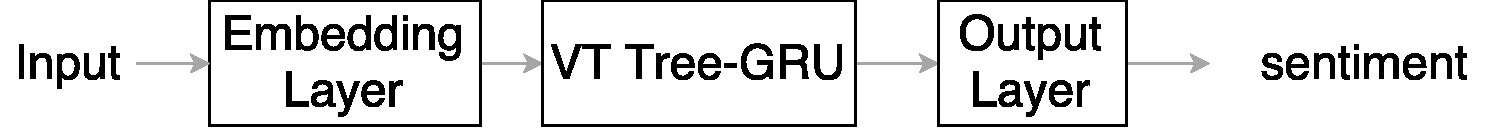
\includegraphics[width=0.8\linewidth]{figure/vtgrusummary.pdf}
    \caption[]{TE Tree-GRU overview}
    \label{fig:vtgrusummary}
\end{figure}

\subsubsection{Embedding layer}\label{sec:embedding}
Embedding layer is a lookup table that converts input data (such as text) into its vector representation. A word embedding layer parameters is its embedding matrix $M  \in \mathbb{R}^{n \times d}$, where $n$ and $d$ is vocabulary size and embedding vector dimension, respectively. In practical, an embedding layer also comes with a vocabulary-index lookup table, which maps words with indexes, which has vector representation corresponding to the row in word embedding matrix.
  
The following steps are required once for each experiment:
\begin{itemize}
    \item Build vocabulary-index lookup table
    \item Init/Load word embedding matrix corresponding to vocabulary-index table
    \item Convert every sentence in dataset into indices using vocabulary-index table  
\end{itemize}
Usually, indices are kept as dataset. Raw dataset (such as readable words) are discarded to free up memory. For each mini-batch, we use indices to look up word representation vector from embedding matrix. Embedding matrix represents of each sentence in dataset are not saved and needed look-up every mini-batch for the following reason.
\begin{itemize}
    \item Saved embedding matrix for each data sentences cost more memory than saving only indices and look-up in embedding layer.
    \item Embedding matrix contains trainable parameters and being updated every iteration.
\end{itemize}

Fig.\ref{fig:embeddinglayer} illustrates embedding layer component and describes the process of convert raw data sentence into its word representation.

\begin{figure}[H]
    \centering
    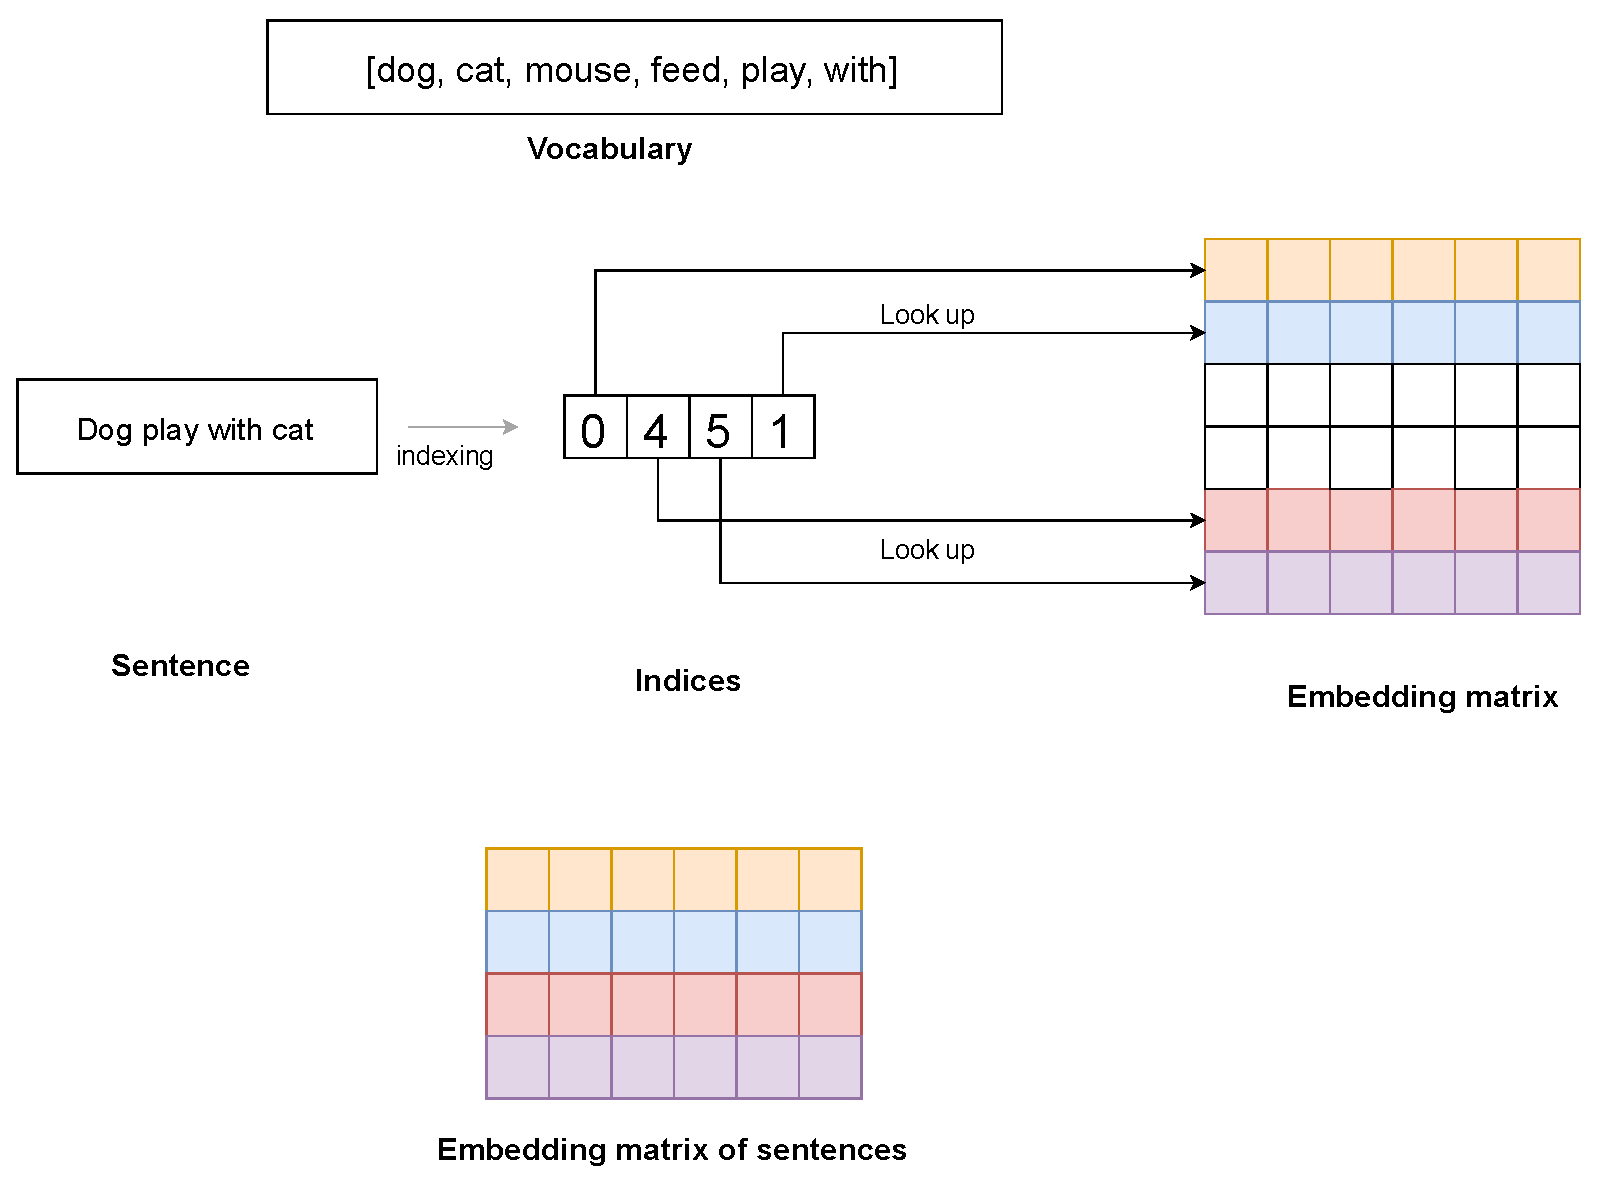
\includegraphics[width=0.9\linewidth]{figure/embeddinglayer.pdf}
    \caption[Overview of embedding layer]{Overview of Embedding Layer}
    \label{fig:embeddinglayer}
\end{figure}



\subsubsection{TE-Tree-GRU}
We applied both tree structure network and recurrent structure in our model. 
In each sub-tree, which consists of one parent node with or without children, we applied recurrent network structure over current node and all its child. 
We stored the last hidden layer as node intermediate information and use as input to higher level. 
For network unit, we chose \hyperref[sec:GRU]{Gated Recurrent Unit (GRU)}~\cite{cho2014learning}. 
GRU transition equations used in our implementation are describe in Eq.\ref{eq:gru}. 

\begin{equation}
\label{eq:gru}
\begin{aligned}
&r = sigmoid(W_{ir} x + b_{ir} + W_{hr} h + b_{hr}) \\
&i = sigmoid(W_{ii} x + b_{ii} + W_{hi} h + b_{hi}) \\
&n = \tanh(W_{in} x + b_{in} + r * (W_{hn} h + b_{hn})) \\
&h' = (1 - i) * n + i * h\\
\end{aligned}
\end{equation}

\subsubsection{Constituency TE-Tree-GRU} \label{sec:VTtreeConstituency}
SST (Sec.\ref{sec:sst}) given format is binary constituency parse tree. We used CoreNLP~\cite{manning2014stanford} to create non-binary constituency parse tree and annoted Part-of-speech tag (POS-tag) for each node. We then used word and tag and tree structure as input for our model.

For each sub-tree, we sorted child node from left to right order. We took node state k, node POS-tag, and parent POS-tag as input for GRU timestep. We put parent node at the end of GRU chain. We took hidden state of the last timestep as node state k for parent node. For each sub-tree (Fig.\ref{fig:treecp}), model is illustrate in Fig.\ref{fig:cvtgru}. For leaf node case, we inputted word and tag into GRU and got hidden output h as k for leaf node as Fig.\ref{fig:gruleaf}.
\begin{figure}[H]
    \centering
    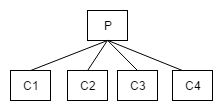
\includegraphics[width=0.5\linewidth]{figure/treecp}
    \caption[A sub tree with parent and children node]{A sub tree with parent and children node}
    \label{fig:treecp}
\end{figure}

\begin{figure}[H]
    \centering
    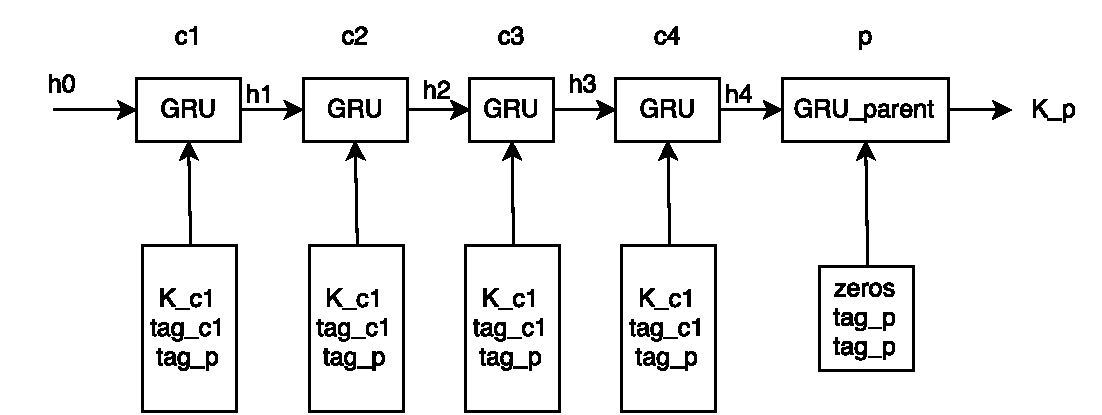
\includegraphics[width=0.9\linewidth]{figure/cvtgru}
    \caption[Constituency TE-Tree-GRU]{Constituency TE-Tree-GRU}
    \label{fig:cvtgru}
\end{figure}

\begin{figure}[H]
    \centering
    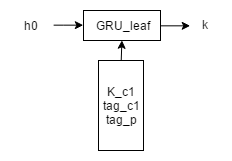
\includegraphics[width=0.4\linewidth]{figure/gruleaf}
    \caption[Constituency TE-Tree-GRU leaf case]{Constituency TE-Tree-GRU leaf case}
    \label{fig:gruleaf}
\end{figure}



\subsubsection{Dependency TE-Tree-GRU} \label{sec:VTtreeDependency}
We used~\cite{manning2014stanford} to create dependency parse tree with annotated POS-tag and labeled Universal Dependencies between head word and its dependents.

We built a model similar to constituency case, with a chain GRU for each sub tree. However, we did not put parent node at the end of the chain. Instead, parent node and child node were sorted according to their position in sentences. We took node state k, node POS-tag, node dependency relationship type vs head word as input for GRU timestep. At parent node, we set dependency relationship type is 'self' and node states k set to zeros vector. We took hidden state of the last timestep as node state k for parent node. In case of leaf node, we treated it as parent node without children. We built GRU chain with only parent node for leaf case. Fig.\ref{fig:dependencyvtgru} illustrates Dependency TE GRU model.

\begin{figure}[H]
    \centering
    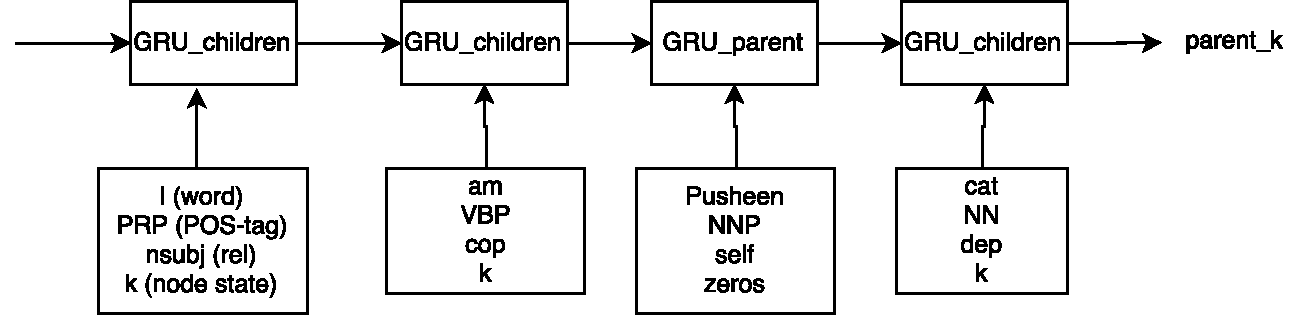
\includegraphics[width=0.9\linewidth]{figure/dependencyvtgru}
    \caption[Dependency TE-Tree-GRU]{Dependency TE-Tree-GRU}
    \label{fig:dependencyvtgru}
\end{figure}

\subsubsection{Output layer and loss function}
We used softmax classifier and cross entropy loss function as described in~\cite{treeLSTM}.  For each parent labeled node, we used node state $k$ as input to output layer and calculate loss against given label. Root node state $k$ was used to determine sentiment of whole sentences.
\subsection{Training method and hyper-parameters}
We preprocessed SST as described in Sec.\ref{sec:VTtreeConstituency} and Sec.\ref{sec:VTtreeDependency}. We used default train/dev/test split after removing neutral sentences (6920/872/1821). We only remove neutral sentence but keep neutral text span of positive or negative sentences. We fine tune our model on development dataset using grid search.

We initialized our word representation with pretrained word vector (Glove\footnote{Common Crawl (840B tokens, 2.2M vocab, cased, 300d vectors, 2.03 GB download) publicly available at \url{https://nlp.stanford.edu/projects/glove/}}~\cite{glove})  with default dimension of 300.  We initialize randomly tag and relationship representation (dependency only) vector of dimension 50. We set memory dimensions of 150. 

Our model was trained using AdaGrad~\cite{duchi2011adaptive} with learning rate of $\{0.1,~ 0.05,~ 0.01\}$ and Adam $\{1e^{-3}, 1e^{-4}\}$, L2 regularization strength of $\{1e^{-3},~ 1e^{-4}, ~ 1e^{-5} \}$, batch size of 25. We manually updated our word representation with learning rate $\alpha$ of $\{0.1,~0.05, ~0.01\}$ as Eq.\ref{eq:manuallyupdate}. In addition, we used dropout~\cite{krizhevsky2012imagenet} to regularize our model. We regularized Tree-GRU with input dropout rate of 0.5 and memory dropout rate at 0.1. Sentiment classifier was also regularized with 0.5 dropout rate. 

\hypertarget{sec:Glove-Amazon}{\section{Training Glove embedding on Amazon reviews dataset}}
\label{sec:gloveamazone}
\subsection{Steps for preprocessing Amazon dataset for training Glove vectors}
\label{sec:preprocessamazonglove}
\begin{enumerate}
\item For retraining Glove vectors, we only used Amazon Movies and TV reviews dataset (7,850,072 reviews)~\cite{mcauley2013hidden}, Amazon Book reviews(22,507,155 reviews) and new Movies and TV dataset (4,607,047 reviews)~\cite{McAuleyTSH15}~\cite{HeM16}.
\item All the reviews were grouped by product-ID ("asin" keyword in the \hyperref[sec:amazon]{JSON schema of the dataset}). 
\item In each product-ID group, the reviews were sorted increasingly by their rating ("overall" keyword in the JSON schema of the dataset).
\item All the reviews were dumped into a plain text file.
\item The text file produced from the previous step was tokenized using Stanford Tokenizer~\cite{tokenizerpart}. 
\end{enumerate}
The reason for doing step 2 and step 3 is because there is no definition of end-of-document in Glove model, which means words which appear in the beginning part of a document will be included in the context of words in the last part of the previous document, this lead to noise in training data, step 2 and 3 help us to mitigate this problem. 

\subsection{Training method and hyper-parameters}
We use Glove implementation\footnote{Publicly available on Github \url{https://github.com/stanfordnlp/GloVe}} to train word representation. 
We set $x_{max} = 100$, vector size to 300, windows size to 20 and the minimum number of word occurrences to be included in the vocabulary to  5.
The training process took the plain text file produced by the \hyperref[sec:preprocessamazonglove]{preprocessing steps} as its input. 
In total, the size of the corpus is 4.7 billions tokens. 
After the training process, the resulting word embeddings has vocabulary size of 1,734,244.
We named this word embeddings Glove Amazon. 
Apart from using Glove Amazon to replace Glove Common Crawl for initializing word embedding layer of Tree-LSTM, the whole training process and hyper-parameters are kept unchanged (Sec.\ref{sec:treelstm}).

\hypertarget{sec:CNNtree}{\section{Combining Recusive Neural Networks with Convolution Neural Networks}}\label{sec:CNNtree}
\subsection{Model Description}
\begin{figure}[H]
    \centering
    
\includegraphics[width=0.8\linewidth]{figure/convtreelstmsummary}
    \caption[Convolution Tree-LSTM overview]{Convolution Tree-LSTM overview}
    \label{fig:convtreelstmsummary}
\end{figure}
For this approach, we do experiment with two network architects:
\begin{description}
\item[CNN Tree-LSTM] Given the Constituency Tree-LSTM architect described in Sec.\ref{sec:treelstm},  we inserted a convolution layer between the word embedding layer and the Tree-LSTM's leaf-module.
The rest of TreeLSTM implementation was kept unchanged.
A diagram of CNN Tree-LSTM's modules can be found in Fig.\ref{fig:convtreelstmsummary}.
\item[CNN LSTM] Similar CNN Tree-LSTM but the Tree-LSTM module is replaced by sequential LSTM and a max-pooling layer is added between the convolution layer and LSTM unit.\footnote{Although CNN LSTM seem similar to \hyperref[cnn-rnn]{CNN-RNN}~\cite{cnn-rnn}, we extended it for multichannel input and unsupervised pre-train it. We will explain these techniques in more details in Sec.\ref{sec:model-enhan}} 
One advantage of CNN-LSTM compared to CNN Tree-LSTM is that CNN-LSTM can be unsupervised pre-trained as Language Model, while CNN Tree-LSTM can not (Sec.\ref{sec:unsupervised-pretrain}).
\end{description}


\subsubsection{Convolution layer implementation} \label{sec:conv1c}
Our implementation follows the convolution layer described in Sec.\ref{kim-cnn}.
Each convolution layer contains n filter. 
Each filter has dimension $wd$, with \(d\) is word vector dimensions and \(w\) is word-level kernel size. 
The number of kernel and the size of each kernel are treated as hyper-parameters 

We aligned the first axis of each feature map with the embedding axis and convolved along the first dimension of embedding matrix. 
We used 'half' convolutions~\footnote{'half' padding policy: http://deeplearning.net/software/theano/tutorial/conv\_arithmetic.html} with unit strides, which each filter produce a 1d vector have which have the same length as the input sentence length. 
Thus, n filters produce a $l \times n$ matrix with $l$ is sentence length. 
We used ReLU activation function~\cite{hahnloser2000digital}. Fig \ref{fig:convlayer} illustrates convolution process. 



\begin{figure}[H]
    \centering
    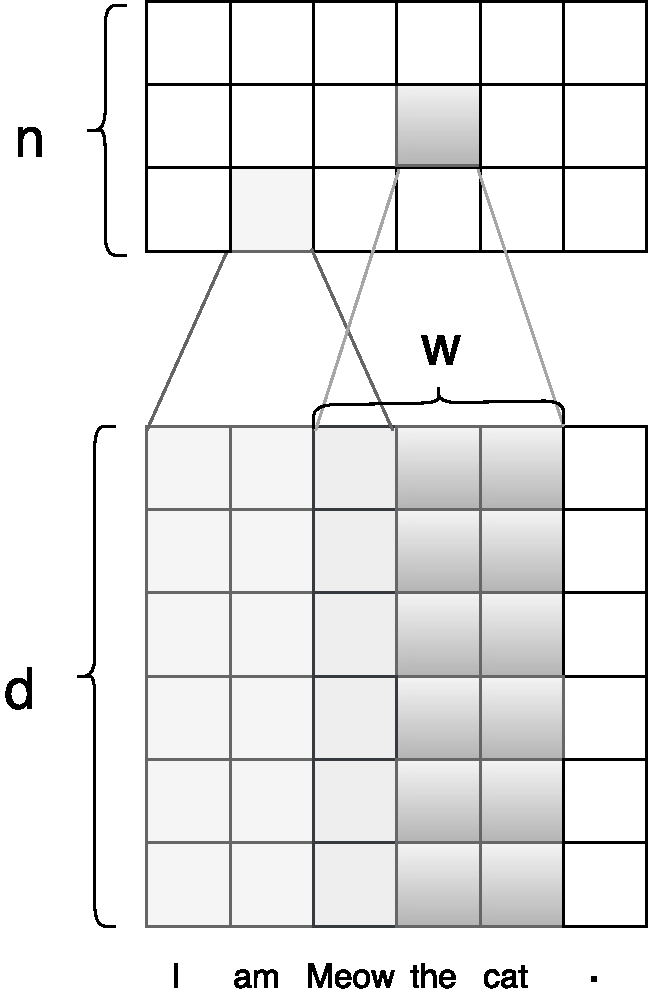
\includegraphics[width=0.4\linewidth]{figure/convlayer}
    \caption[Convolution layer]{Convolution layer}
    \label{fig:convlayer}
\end{figure}

\subsection{Models Enhancements}\label{sec:model-enhan}
\subsubsection{Training Glove embedding on Amazon reviews dataset}\label{sec:reuse-glove-amazon}
We reused Glove Amazon word embedding (Sec.\ref{sec:gloveamazone}).

\subsubsection{Using multi-channel word embeddings}\label{sec:enhan-multi-channel}
This method was introduced by Yoon Kim~\cite{KimCNN}.
The description and analysis of this method can be found in Sec.\ref{kim-cnn}.
Although in his paper, in the training process of his 2-channel-CNN, Kim updated one channel and kept the other unchanged, we are not restricted ourselves to this rule. 
The type of word embeddings used in each channel, the number of channels and the method for updating each channel are treated as hyper-parameters.

This method allows multiple parallel embedding layers in our model. 
In other words, each word is presented by multiple vector representations. 

\begin{figure}[H]
    \centering
    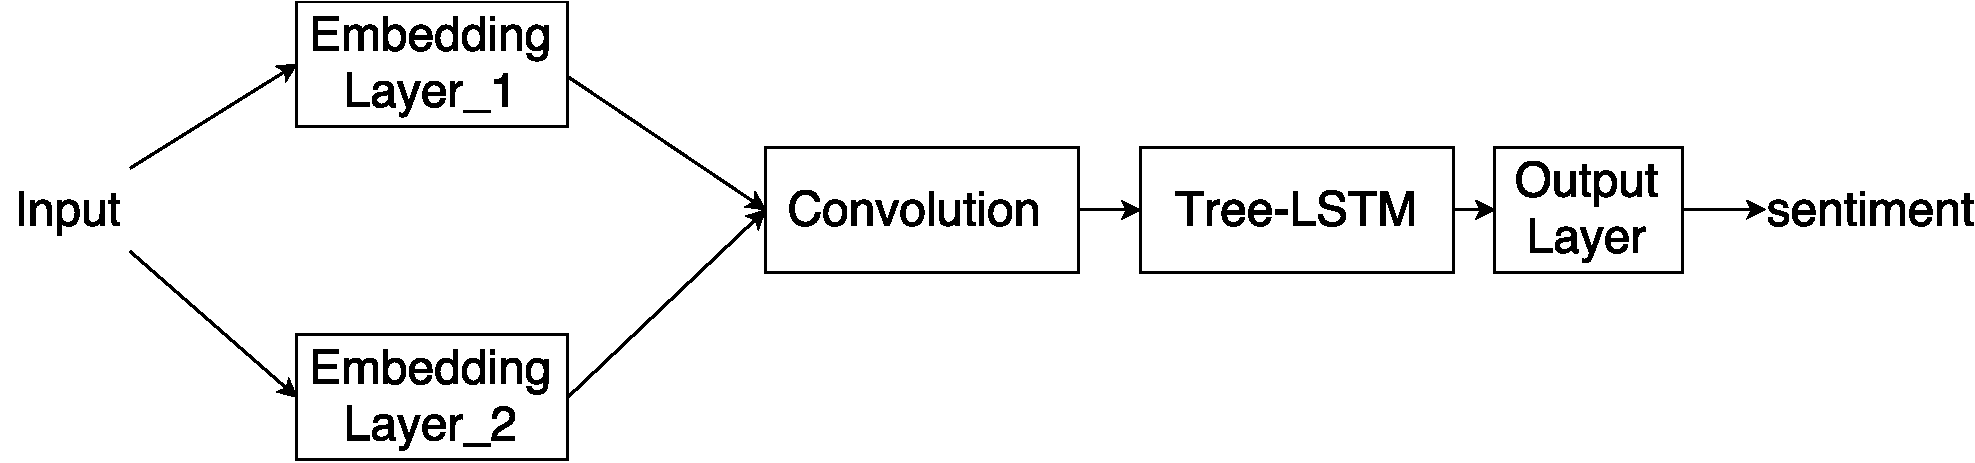
\includegraphics[width=0.8\linewidth]{figure/multichannelcnnlstm}
    \caption[Convolution Tree-LSTM overview]{Two input channel Convolution Tree-LSTM overview}
    \label{fig:multichannelcnnlstm}
\end{figure}


\subsubsection{Pre-training models on Amazon reviews dataset}
\label{enhan-unsupervised-pretrain}
We presented several methods for unsupervised pre-training neural network models and given some hypotheses on the beneficial effects of these methods in Sec.\ref{sec:unsupervised-pretrain}.
\paragraph{Steps for preprocessing Amazon dataset for training Language Model}
\label{sec:preprocessamazonglove-LM}
\begin{enumerate}
\item For retraining Glove vectors, we only used new Movies and TV dataset (4,607,047 reviews)~\cite{McAuleyTSH15}~\cite{HeM16}.
\item All the reviews were grouped by product-ID ("asin" keyword in the \hyperref[sec:amazon]{JSON schema of the dataset}). 
\item In each product-ID group, the reviews were sorted increasingly by their rating ("overall" keyword in the JSON schema of the dataset).
\item A special character sequence was added at the end of each review to mark its end.
After that, all the reviews were dumped into a plain text file.
\item The text file produced from the previous step was tokenized using Stanford Tokenizer~\cite{tokenizerpart}. 
\item The tokenized text file was then divided into training and test set using 95:5 split.
As this is a pre-training process, we used only 5\% of the data to test if the Language Model was trained properly.
\end{enumerate}

Step 2, 3 and 4 are for mitigating the problem of noise in training data which have been presented in Sec.\ref{sec:preprocessamazonglove}.

\subsection{Training method and hyper-parameter}
For the models with only single input channel, we initialized word representation with Glove vectors~\cite{glove}. 
With two word embeddings channels, we initialized one channel using Glove Common Crawl\footnote{\label{glovecommoncrawl}Common Crawl (840B tokens, 2.2M vocabularies, cased, 300d vectors, 2.03 GB download) publicly available at \url{https://nlp.stanford.edu/projects/glove/}} and the other using our Glove Amazon (Sec.\ref{sec:reuse-glove-amazon}). 

We tried a variety of convolution filters combination. 
For single kernel size, we performed grid search on $\{100, 200, 300\}$ number of kernels of size $\{3, 5\}$. 
For two different kernel size, we tried with $\{100, 200\}$ number of kernels for each kernel size. 
Output matrices of different kernel sizes were concatenated as if they were with same kernel size. 

Our model was trained using AdaGrad~\cite{duchi2011adaptive} with learning rate of $\{0.1,~ 0.05,~ 0.01\}$, L2 regularization of $\{1e^{-3},~ 1e^{-4}, ~ 1e^{-5} \}$, batch size of 25. 
We manually update our word representation with learning rate $\alpha$ of $\{0.1,~0.05, ~0.01\}$ following Eq.\ref{eq:manuallyupdate}. 
We regularized convolution layer with input dropout rate of 0.5 and output dropout rate of 0.2 in addition to dropout of rate 0.5 at dropout layer. 
We applied the same hyper-parameters grid search for two channels convolution. 
\begin{equation}
\label{eq:manuallyupdate}
w = w - \alpha\delta J(\theta)
\end{equation}
